%
\chapter{Fundamentals}\label{cha:Fundamentals}
%
%Eine wissenschaftliche Abschlussarbeit kann im Allgemeinen in die folgenden 4 Phasen gegliedert werden.
%
\section*{2.1.Properties of Truck at Carolo-Cup}
\label{sec:Properties of Truck at Carolo-Cup}
\addcontentsline{toc}{section}{2.1.Properties of Truck at Carolo-Cup}
%

The Carolo-Cup is an annual competition at the Technical University of Braunschweig 
which are attended by student. Every year the truck and some properties of the 
competition is changing. For example, in the competitions until 2017 there was no 
traffic sign but from 2017 there are also some traffic signs, speed limit zones, 
blocked areas and crosswalks with pedestrian. Because of this reason, in the 
competitions until 2017, there was only one way to understand who has the right of way. 
If there is a stop line in the way which in front of intersection, it means, the car 
has to wait until the intersection is free. In the competitions from 2017, the 
intersections are in different parts: They are 'Intersections with stop lines', 
'Intersections with give-way lines', 'Intersections with priority to right', 
'Enforced crossing direction - give-way condition', 'Enforced crossing direction - 
right of way condition'. Except 'Intersections with priority to right', they all have 
traffic signs, which signs who has priority. If there is a no traffic sign, it means,
right side always have priority.



\begin{figure}[H]
	\centering
	\hspace*{0cm}   
	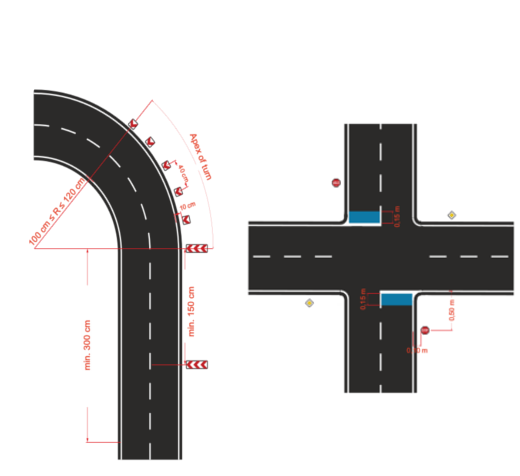
\includegraphics[width=120mm,scale=1]{./Bilder/Intersections.png}
	\caption{Left: Markings for sharp turns at Carolo-Cup.
Right: Intersections with stop lines at Carolo-Cup}
\end{figure}


%
\section*{2.2. Inverse Perspective Mapping}\label{sec:Inverse Perspective Mapping}
\addcontentsline{toc}{section}{2.2. Inverse Perspective Mapping}
%
Inverse Perspective Mapping(IPM) is an algorithm which obtain accurate bird's-eye view images from the sequential 
of forward looking cameras. At IPM algorithm, each image pixel is re-mapped, and a new array of pixels is created 
where the lines in perspective are transformed into straight lines and objects are distorted. IPM is one of the 
most used methods at lane detection. At lane detection, IPM ensures to show the lanes vertical and parallel to 
each other. On the other hand, because of re-mapping of pixels, IPM is a computationally expensive method. Because 
of this reason, in this master thesis, in some methods, except to remap the all pixels of images, just the pixels,
which are relevant to lane and accordingly the fitted curve were remapped. Thanks to this, in some methods, so many 
time of computing was saved.

For using IPM method, the intrinsic and extrinsic parameters of camera are necessary to process images for coordinate 
transformation and calibration. 

\begin{itemize}
 \item \textbf{Intrinsic Parameters :} Instrinsic parameters include are specific to a camera. It includes information
of the focal length ($f_x$, $f_y$) and optical centers ($c_x$, $c_y$). It is also called camera matrix. It depends on 
the camera only, so once calibrated, it can be stored for future purposes. It is expressed as a 3x3 matrix: 

 \begin{center}
  camera matrix =  $
 \begin{bmatrix} 
f_x & 0 & c_x \\
0 & f_y & c_y \\
0 & 0 & 1 \\
\end{bmatrix}
$  \end{center}

 \item \textbf{Extrinsic Parameters :} Extrinsic parameters are relevant with the camera position. The parameters are H 
 and $\theta$. H is the distance between the camera and ground. $\theta$ is the camera tilt angle. 
 
  \end{itemize}
  
 \begin{figure}[H]
	\centering
	\hspace*{0cm}   
	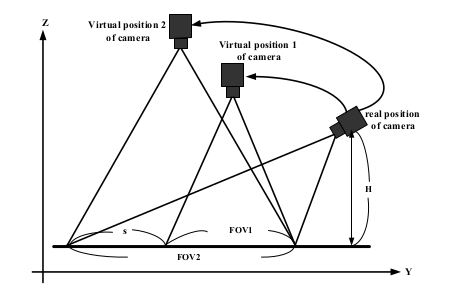
\includegraphics[width=150mm,scale=1]{./Bilder/Related_positions_of_the_camera.png}
	\caption{Related Positions of the Camera \cite{IPM}}
\end{figure}
 
 As seen at Abbildung 2.2, the camera on the car has field of view 2(FOV2) at its real position of camera but in this 
 case, the view is not bird-eye view so if the same FOV want to be seen from bird-eye view, IPM will virtually change
 the position to Virtual position 2 of camera. In this case, although the camera is at its real position, it will look
 like that it is at the virtual position 2. For that, the image coordinates must be also changed. Below, steps of IPM 
 calculations will be from the paper of \cite{IPM} described.
 
 In the formula, original image coordinates will be defined as (x,y), the destination image coordinates will be 
 defined as ($x^*$,$y^*$), the distance between ground and camera will be defines as H, the focal length of camera 
 will be defines as f and the tilt angle of camera will be defined as $\theta$.
 
\begin{center}
 $x^* = H \frac{x sin \theta + f cos \theta}{-y cos \theta + f sin \theta}$ ;
 $y^* = H \frac{y sin \theta + f cos \theta}{-y cos \theta + f sin \theta}$ 
\end{center}

In this equation , the transformed component values of $x^*$ and $y^*$ may be less than or equal to zero. Because of 
this reason, a constant d is defined as $
\begin{vmatrix}
H(sin \theta + cos \theta)/(f sin \theta - cos \theta) 
\end{vmatrix}
$  + 1. This means that the coordinate point in the original source image has been mapped into the point of  the 
destination image coordinate system. Below there is the proposed equation :
 
 \begin{center}
 $x^* = H \frac{x sin \theta + f cos \theta}{-y cos \theta + f sin \theta}$ + d ,
 $y^* = H \frac{y sin \theta + f cos \theta}{-y cos \theta + f sin \theta}$ + d ,
 where d = 
 $\begin{vmatrix}
 \frac{H(sin \theta + f cos \theta)}{f sin \theta - cos \theta}
 \end{vmatrix}$ + 1
\end{center}

\begin{figure}[H]
	\centering
	\hspace*{0cm}   
	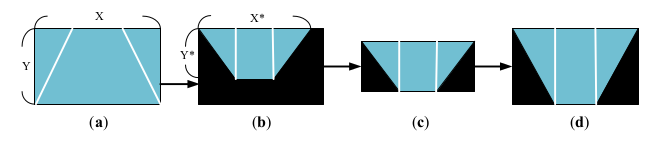
\includegraphics[width=170mm,scale=1]{./Bilder/Procedures_of_IPM.png}
	\caption{Procedures of IPM \cite{IPM}}
\end{figure}

%
\section*{2.3. Edge Detection}\label{sec:Edge Detection}
\addcontentsline{toc}{section}{2.3. Edge Detection}
%
Edge detectors are essential parts of most of computer vision systems. Edge detectors decrease dramatically the 
amount of data to be processed and extract the useful part of images. They work by detecting discontinuities in 
brightness.  In this project, the edge detector was used, the lanes to detect and prevent unnecessary information 
from images.There are different methods for edge detection but it can be grouped in two categories. They are :



\begin{itemize}

\item \textbf{Gradient method : } This method searches the maximum and minimum in the first derivative of the image 
and within can find the edges. For this method, first order derivative filter must be used. For example : Sobel 
Operator.
 
\item \textbf{Laplacian method : } This method searches for zero crossing in the second derivative of the image 
and within can find the edges. For this method, second order derivative filter must be used. For example : 
Laplacian Filter.
  
 \end{itemize}
 
According to \cite{Machine_Vision},there are three steps at edge detection algoritm. They are :
\begin{itemize}
 \item \textbf{Filtering : } For edge detection, it is required to use an suitable smoothing filter. The filters 
 sharpen the edges and inhibit the unnecessary informations. It is often utilized to improve the functioning of 
 an edge detector against noise. The more filtering is applied, however, the greater the loss of edge strength.
 
 \item \textbf{Enhancement : } To be able to better detect edges, changes in the intensity in the area 
 surrounding a point must be determined. Pixels in which a significant change in intensity occurs are 
 emphasized by enhancement, which is usually applied by calculating the gradient magnitude.
  
 \item \textbf{Detection : } Though many points in an image have a nonzero value for the gradient, not all of 
 these points are actually edges. Because only points with strong edge content are desired, a method must be 
 applied to determine which points are actual edge points. Thresholding is often utilized to do so.
 
\end{itemize}



Well known smoothing filters are :

\begin{itemize}
 \item Sobel-Operator
 \item Canny Edge Detector
 \item Laplacian-Filter
 \item Prewitt-Operator
 \end{itemize}
 
 In this master thesis, Sobel Operator were used so it will be described a bit in detail.
%
\subsection*{2.3.1. Sobel Operator}\label{sec:Sobel Operator}
\addcontentsline{toc}{subsection}{2.3.1. Sobel Operator}

The Sobel Operator uses vertical and horizantel masks. These masks are used odd-sized square matrices and 
they are generally 3x3 matrices.
%
\section*{2.4. Hough-Transformation}\label{sec:Hough - Transformation}
\addcontentsline{toc}{section}{2.4. Hough - Transformation}
%

%
\subsection*{2.4.1. Standart Hough - Transformation}\label{sec:Standart Hough - Transformation}
\addcontentsline{toc}{subsection}{2.4.1. Standart Hough - Transformation}
%


%
\subsection*{2.4.2. Probabilistic Hough - Transformation}\label{sec:Probabilistic Hough - Transformation}
\addcontentsline{toc}{subsection}{2.4.2. Probabilistic Hough - Transformation}
%




%
\section*{2.5. K-Nearest Neighbors}\label{sec:K-Nearest Neighbors}
\addcontentsline{toc}{section}{2.5. K-Nearest Neighbors}
%



%
\section*{2.6. Curve Fitting}\label{sec:Curve Fitting}
\addcontentsline{toc}{section}{2.6. Curve Fitting}
%

%




